\documentclass{article}

\usepackage{arxiv}

\usepackage[utf8]{inputenc}
\usepackage[T1]{fontenc}
\usepackage{hyperref}
\usepackage{url}
\usepackage{booktabs}
\usepackage{amsfonts}
\usepackage{amsmath}
\usepackage{amssymb}
\usepackage{nicefrac}
\usepackage{microtype}
\usepackage{graphicx}
\usepackage{xcolor}
\usepackage{algorithm}
\usepackage{algpseudocode}
\graphicspath{ {./images/} }

% ---------------------------------------------------------------
\title{Block-Sparse Attention with Prefix Caching: Integrating
       MInference into vLLM via the PagedAttention--Sparsity Isomorphism}

\author{
  Anton Po \\
  University of Macau \\
  \texttt{dc22762@um.edu.mo} \\
}

\begin{document}
\maketitle

% ---------------------------------------------------------------
\begin{abstract}
Dynamic block-sparse attention, as demonstrated by MInference
\cite{minference}, significantly accelerates the pre-filling stage of
long-context Large Language Model (LLM) inference by exploiting the
observation that attention weight matrices are highly sparse in practice.
However, the original MInference implementation operates under a strict
assumption: query, key, and value sequences must share identical lengths,
precluding its use with KV cache---the standard mechanism by which
production inference systems avoid recomputing past context. This
limitation means MInference cannot natively benefit from prefix caching,
a key feature of vLLM \cite{pagedattention} that eliminates redundant
computation for shared system prompts.

This work identifies and formalises a structural isomorphism between the
block-sparse attention grid and PagedAttention's paged memory layout: an
attention block indexed by column $c$ directly corresponds to the physical
KV page $\phi(c)$ in PagedAttention's block table. This natural alignment,
previously unrecognised, means that block-sparse attention is
\textit{inherently compatible} with paged memory management---no data
reorganisation or auxiliary structures are required. By integrating the
block-sparse importance predictor of MInference into the vLLM inference
framework, prefix-cached KV pages can be selectively attended to based on
predicted block importance, enabling MInference-style sparsity to
coexist with prefix caching for the first time. The approach further
integrates with FlashAttention's online softmax formulation
\cite{flashattention2}, preserving numerical correctness. Experiments
demonstrate up to a 63\% reduction in attention kernel latency at 100K
tokens with a 90K token prefix cache, with output tensors numerically
near-identical to the MInference baseline.
\end{abstract}

% ---------------------------------------------------------------
\section{Introduction}
\label{sec:intro}

State-of-the-art Large Language Models (LLMs) increasingly demand
long-context reasoning capabilities, with context windows now spanning 128K
to 10M tokens \cite{minference, geminiteam2024gemini15unlockingmultimodal}.
A particularly common deployment pattern is the use of long system
prompts \cite{zheng2024sglang}---detailed instructions, retrieved documents,
or shared conversational context---that remain identical across many user
requests. In such settings, the transformer must repeatedly process the same
lengthy prefix for every new query, recomputing the associated Key-Value (KV)
cache from scratch each time. This redundant recomputation becomes
increasingly expensive as context length grows: for a prompt of $1\text{M}$
tokens, attention computation alone can account for over 90\% of total
pre-filling latency \cite{minference}, making repeated recomputation of long
shared prefixes a fundamental bottleneck in production LLM inference.

Two complementary lines of work have independently addressed aspects of this
bottleneck. \textbf{PagedAttention} \cite{pagedattention}, implemented in
vLLM, addresses the memory management side: it stores KV caches in
fixed-size physical blocks and supports \textit{prefix caching}, which
allows the KV cache of a shared prefix to be computed once and reused
across all subsequent requests, eliminating redundant recomputation
entirely. Prefix caching has become a standard feature in modern LLM
serving frameworks---both vLLM \cite{pagedattention} and SGLang
\cite{zheng2024sglang} enable it by default---and is widely regarded as
one of the most impactful optimisations for serving workloads with repeated
long prompts. \textbf{MInference} \cite{minference} addresses the computation
side: it demonstrates that attention weight matrices are highly sparse in
long-context LLMs, and exploits this sparsity to skip up to 95\% of
attention FLOPs during pre-filling via dynamic block-sparse attention.
Despite these advances in the serving ecosystem, MInference does not
support prefix caching and cannot benefit from the KV cache reuse that
vLLM \cite{pagedattention} and SGLang \cite{zheng2024sglang} provide.

Despite their complementary goals, these two systems are currently
\textit{incompatible}. When new tokens arrive, their query, key, and value
projections ($Q$, $K$, $V$) are computed from the new token embeddings
alone---so $Q$, $K$, and $V$ for the new tokens all share the same length
$n_q$. However, for attention to be correct, the new queries must attend
over \textit{all} context: both the new tokens and the full cached prefix.
This requires the attention kernel to accept the cached KV as a separate
input and concatenate it with the new-token KV before computing attention.

MInference's block-sparse kernel was not designed for this. It operates
under the assumption that the entire context is processed from scratch in a
single pre-filling pass---a single $Q$, $K$, $V$ of uniform length $n$
covering all tokens together. It has no mechanism to accept a pre-computed
external KV cache as a separate input, combine it with new-token KV
internally, and apply block-sparse selection over the resulting combined
sequence. As a result, the only way to use MInference is to recompute the
full context---prefix and new tokens together---from scratch on every
request, which entirely defeats the purpose of prefix caching. MInference
is therefore incompatible with KV cache reuse in any form.

This work closes that gap by identifying a fundamental structural property
that has been overlooked: \textbf{block-sparse attention is naturally
compatible with PagedAttention's paged memory layout by design}. The
attention matrix is partitioned into blocks of size $b \times b$, exactly
mirroring PagedAttention's physical blocks of $B$ tokens. An attention
block at column index $c$ requires precisely the KV vectors stored in
physical page $\phi(c)$ of PagedAttention's block table---a one-to-one
correspondence that requires no data reorganisation, no auxiliary index
structures, and no modification to the block table itself. This isomorphism
means that block-sparse attention can operate directly over paged KV caches,
selectively attending only to the pages whose block importance scores are
above the top-$k_b$ threshold, while prefix-cached pages that are not
selected are simply skipped.

The main contributions of this work are as follows:
\begin{enumerate}
  \item The fundamental incompatibility of existing sparse attention methods
    with KV cache is identified, with MInference's equal-length QKV
    constraint as the primary barrier to prefix caching support.
  \item The structural isomorphism between block-sparse attention column
    indices and PagedAttention's physical page addresses is formalised,
    proving that block-sparse attention is natively compatible with paged
    memory management.
  \item The block-sparse importance predictor of MInference
    \cite{minference} is integrated into the vLLM inference framework,
    enabling sparse attention over prefix-cached KV pages for the first time.
  \item Empirical evaluation demonstrates a 63\% reduction in attention
    kernel latency at 100K tokens with a 90K token prefix cache, and
    near-identical output fidelity relative to the MInference baseline.
\end{enumerate}

% ---------------------------------------------------------------
\section{Background}
\label{sec:background}

\subsection{The KV Cache and Prefix Caching}

Autoregressive generation in transformer-based LLMs requires, at each
decoding step $t$, access to all previously computed key and value tensors
$\{K_1, \ldots, K_t\}$ and $\{V_1, \ldots, V_t\}$. Without caching,
recomputing these tensors at each step would incur $O(t^2)$ cumulative
cost. The KV cache stores these tensors persistently, allowing each step
to attend over previously computed context at constant marginal cost.

For a model with $L$ layers, $H$ heads, head dimension $d_h$, and sequence
length $n$, the total KV cache size is:
%
\begin{equation}
  \text{KV Cache Size} = 2 \times L \times H \times d_h \times n
    \times \texttt{sizeof}(\texttt{dtype})
  \label{eq:kvcache-size}
\end{equation}
%
In production deployments, a significant fraction of the KV cache
corresponds to a shared system prompt that is identical across all user
requests. Recomputing this prefix for every new request is wasteful.
\textbf{Prefix caching}, as implemented in vLLM \cite{pagedattention} and
SGLang \cite{zheng2024sglang}, avoids this by storing the computed prefix
KV cache once and reusing it across all requests that share it, reducing
redundant computation proportionally to the prefix length.

\subsection{PagedAttention and vLLM}

PagedAttention \cite{pagedattention} addresses KV cache memory management
through an OS-inspired virtual memory abstraction. Rather than allocating
a contiguous memory region per request, PagedAttention manages the KV cache
in fixed-size, non-contiguous \textbf{physical blocks} of $B$ tokens each
(e.g., $B = 64$). Each request maintains a logical block sequence mapped to
physical blocks via a \textbf{block table}. Formally, let
$\mathcal{B} = \{b_1, b_2, \ldots, b_m\}$ be the set of physical blocks
allocated to a request, and let $\phi: [m] \rightarrow \mathcal{B}$ be the
mapping from logical block indices to physical addresses.

Prefix caching is implemented by marking physical blocks corresponding to
shared prefixes as immutable and reference-counted. Multiple requests
pointing to the same prefix physical blocks share them without copying,
and the KV cache for the prefix is computed only once. This design is
central to this work: the physical block table $\phi$ is the data structure
through which block-sparse attention and paged memory management are unified.

\subsection{FlashAttention and Online Softmax}

Standard attention \cite{vaswani2023attentionneed} computes:
%
\begin{equation}
  \text{Attention}(Q, K, V) = \text{softmax}\!\left(
    \frac{QK^\top}{\sqrt{d_h}}\right) V
  \label{eq:attention}
\end{equation}
%
This requires materialising the $n \times n$ attention matrix in HBM,
incurring $O(n^2)$ memory complexity. FlashAttention
\cite{flashattention,flashattention2} reformulates this as an IO-aware
tiled computation using \textbf{online softmax} \cite{milakov2018onlinenormalizercalculationsoftmax},
which computes the attention output incrementally across tiles without
materialising the full matrix. At each tile step $j$, running statistics
$(m_j, \ell_j, O_j)$ are updated as:
%
\begin{align}
  m_j      &= \max\!\left(m_{j-1},\; \text{rowmax}(S_j)\right)
    \label{eq:online-m} \\
  \ell_j   &= e^{m_{j-1} - m_j} \cdot \ell_{j-1}
             + \text{rowsum}\!\left(e^{S_j - m_j}\right)
    \label{eq:online-l} \\
  O_j      &= \text{diag}\!\left(e^{m_{j-1} - m_j}\right) O_{j-1}
             + e^{S_j - m_j} V_j
    \label{eq:online-o}
\end{align}
%
where $S_j = Q K_j^\top / \sqrt{d_h}$, yielding final output
$O = \text{diag}(\ell_T)^{-1} O_T$.
Crucially, this formulation permits \textit{skipping tiles entirely}:
if a tile is unimportant, omitting it introduces only bounded approximation
error~\ref{sec:error-bound}. This is the mathematical foundation of block-sparse attention.
FlashAttention's IO complexity is $\Theta\!\left(\frac{n^2 d_h^2}{M}\right)$,
where $M$ is the on-chip SRAM size, compared to $\Theta(nd_h + n^2)$ for
standard attention.

\subsection{MInference: Dynamic Block-Sparse Attention}

MInference \cite{minference} demonstrates that attention weight matrices
in long-context LLMs are highly sparse: at any given layer and head, each
token attends to fewer than 5\% of all preceding tokens for sequences
exceeding 128K tokens. This sparsity is dynamic (varies per input) but
\textit{predictable online} from the current $Q$ and $K$ activations
without retraining.

For \textit{Block-Sparse} heads, MInference computes a coarse block-level
attention score via mean pooling of $Q$ and $K$, selects the top-$k_b$
blocks per query row, and executes full-precision attention only over those
blocks---reducing FLOPs by up to 95\% while preserving model quality.

\subsection{Limitation: MInference Does Not Support KV Cache}
\label{sec:limitation}

MInference's block-sparse kernel was designed for the \textit{full
pre-filling} scenario: the entire input context of length $n$---system
prompt, history, and new tokens---is passed as a single uniform $Q$, $K$,
$V$ triplet of identical length $n$, and the block-sparse attention is
computed over this complete sequence from scratch.

This design does not accommodate a KV cache. In a cached inference
setting, the key and value projections for the prefix have already been
computed and stored. The new request provides only the new token
embeddings, from which $Q_{\text{new}}$, $K_{\text{new}}$, and
$V_{\text{new}}$ of length $n_q$ are projected. To compute correct
attention, $Q_{\text{new}}$ must attend over the \textit{full} KV
sequence---the cached prefix KV concatenated with the new-token KV:
%
\begin{equation}
  K_{\text{full}} = [K_{\text{cached}};\; K_{\text{new}}], \quad
  V_{\text{full}} = [V_{\text{cached}};\; V_{\text{new}}]
  \label{eq:kv-concat}
\end{equation}
%
MInference's kernel has no interface for this. It cannot accept
$K_{\text{cached}}$ and $V_{\text{cached}}$ as a separately provided input
and combine them with the new-token projections internally. The kernel
always expects a single contiguous $Q$, $K$, $V$ buffer of uniform length.
The only way to use MInference with a long prefix is therefore to
recompute the prefix KV from its raw token embeddings on every request,
which completely defeats the purpose of prefix caching and eliminates its
latency benefit.

This is a fundamental architectural limitation: MInference cannot be
applied in any deployment that uses a KV cache---which includes virtually
every production LLM serving system, including multi-turn conversation,
RAG pipelines, and shared system prompt scenarios.

% ---------------------------------------------------------------
\section{Block-Sparse Attention: Formulation}
\label{sec:sparse}

\subsection{The Sparsity Observation}

Let $A \in \mathbb{R}^{n_q \times (n_p + n_q)}$ denote the attention
weight matrix for a single head in the prefix caching setting, where
$n_q$ is the query length and $n_p$ the cached prefix length. Partitioning
$A$ into a grid of blocks of size $b \times b$:
%
\begin{equation}
  A^{(r,c)} = A[r \cdot b : (r+1) \cdot b,\; c \cdot b : (c+1) \cdot b],
  \quad r \in \left[0, \lceil n_q/b \rceil\right),\;
       c \in \left[0, \lceil (n_p+n_q)/b \rceil\right)
  \label{eq:block-partition}
\end{equation}
%
This is a \textit{rectangular} block grid, with more column blocks than
row blocks whenever $n_p > 0$. The set of important blocks $\mathcal{I}$
is defined by per-row top-$k_b$ selection over a coarse approximation of
the attention scores, described in Section~\ref{sec:approx}. The key
empirical observation from Jiang et al.\ \cite{minference} is that for
$n > 128\text{K}$, retaining only the top $k_b = 4096$ columns out of
$128{,}000$ already recalls 96.8\% of the total attention
mass---confirming that $|\mathcal{I}| \ll \lceil n_q/b\rceil \cdot
\lceil(n_p+n_q)/b\rceil$ in practice, with the important block count
constituting well under 5\% of the full attention grid.

\subsection{Online Block-Sparse Approximation}
\label{sec:approx}

Since the true attention weights $A$ are unavailable before computation,
the important block set $\mathcal{I}$ is approximated via coarse-grained
pooling. Define:
%
\begin{equation}
  \bar{Q}_r = \frac{1}{b} \sum_{i=rb}^{(r+1)b} Q_i,
  \qquad
  \bar{K}_c = \frac{1}{b} \sum_{j=cb}^{(c+1)b} K_j
  \label{eq:mean-pool}
\end{equation}
%
The block-level coarse attention score is then:
%
\begin{equation}
  \hat{A}_{rc} = \frac{\bar{Q}_r \bar{K}_c^\top}{\sqrt{d_h}}
  \label{eq:coarse-score}
\end{equation}
%
The predicted important block set is selected as the top-$k_b$ blocks per
head across all query rows:
%
\begin{equation}
  \hat{\mathcal{I}} = \text{top-}k_b \text{ blocks of } \hat{A}_{rc}
  \label{eq:topk}
\end{equation}
%
where $k_b$ is a fixed hyperparameter determined offline per head via
kernel-aware search \cite{minference}. Only blocks in $\hat{\mathcal{I}}$
are loaded into GPU SRAM and computed in full precision.

\subsection{Integration with Online Softmax}

The block-sparse computation iterates only over blocks
$(r, c) \in \hat{\mathcal{I}}$ and applies the online softmax update
(Equations~\ref{eq:online-m}--\ref{eq:online-o}) at each step. Since the
online softmax formulation is agnostic to tile ordering and handles
arbitrary subsets of tiles, the sparse iteration is mathematically sound.
Specifically, for query row $r$, the final output satisfies:
%
\begin{equation}
  O_r \approx
  \frac{
    \sum_{c \in \hat{\mathcal{I}}_r} e^{S_{rc} - m_r} V_c
  }{
    \sum_{c \in \hat{\mathcal{I}}_r} e^{S_{rc} - m_r}
  }
  \label{eq:sparse-output}
\end{equation}
%
where $S_{rc} = Q_r K_c^\top / \sqrt{d_h}$ and
$m_r = \max_{c \in \hat{\mathcal{I}}_r} \text{rowmax}(S_{rc})$.
The approximation quality is controlled by $|\hat{\mathcal{I}}_r|$.

% ---------------------------------------------------------------
\section{The PagedAttention--Block-Sparsity Isomorphism}
\label{sec:isomorphism}

\subsection{Why Existing Sparse Attention Cannot Support Paged KV Caches}

Existing sparse attention methods, including MInference, were designed for
the full pre-filling scenario where the entire context is processed as a
single contiguous buffer. This design is incompatible with paged KV caches
in two respects.

First, as established in Section~\ref{sec:limitation}, MInference has no
interface for accepting a pre-computed KV cache as external input. Its
kernel always expects a single $Q$, $K$, $V$ buffer covering the entire
context. To use MInference with a cached prefix, the system must recompute
the prefix KV from raw token embeddings on every request---destroying the
latency benefit of caching entirely. There is no way to ``pass in'' a
stored KV cache and have MInference apply block-sparse selection over the
combined cached-plus-new KV sequence.

Second, even if a KV cache interface existed, the non-contiguous physical
memory layout of PagedAttention would pose an additional barrier. In a
paged cache, the KV vectors for the prefix are scattered across
non-contiguous physical blocks managed by the block table $\phi$. A kernel
that assumes a contiguous KV buffer cannot directly index into this layout
without a costly gather operation that would reassemble the scattered pages
into a flat buffer---adding memory overhead and negating the benefits of
the paged design.

The net result is a structural incompatibility: sparsity-based acceleration
cannot coexist with prefix caching under the existing MInference design.
This has prevented any production inference system from combining these two
optimisations.

\subsection{Block-Sparse Attention is Naturally Compatible with Paged Memory}

The central observation of this work is that \textbf{block-sparse attention
resolves both incompatibilities simultaneously}, without any modification
to the PagedAttention block table or the physical memory layout.

The key insight lies in the correspondence between the unit of computation
in block-sparse attention and the unit of storage in PagedAttention. In
block-sparse attention, the attention matrix is partitioned into blocks of
size $b \times b$, where each block column $c$ spans key-value tokens
$[c \cdot b,\; (c+1) \cdot b)$. In PagedAttention, physical blocks of
size $B$ tokens are managed by the block table $\phi$, where page $\phi(c)$
stores the KV vectors for tokens $[c \cdot B,\; (c+1) \cdot B)$.

Setting $b = B$, the correspondence is exact and complete:

\begin{center}
\textit{The KV vectors required to compute attention block $(r, c)$ are}\\
\textit{precisely the vectors stored in physical page $\phi(c)$.}
\end{center}

This yields a direct structural isomorphism:
%
\begin{equation}
  \text{Attention Block } (r, c)
  \;\longleftrightarrow\;
  \text{Physical KV Page } \phi(c)
  \label{eq:isomorphism}
\end{equation}
%
The column index $c$ in the sparse attention block grid is \textit{the same
index} used to look up the physical page in PagedAttention's block table.
No translation layer, no gather operation, and no data reorganisation are
required. The block table $\phi$ already provides $O(1)$ access to the
exact physical memory needed for any given attention block.

This resolves the KV cache interface problem as well. The new-token
query $Q_{\text{new}}$ attends over the full key-value sequence
$K_{\text{full}} = [K_{\text{cached}};\; K_{\text{new}}]$, whose blocks
map directly onto the block table: prefix pages
$\{\phi(0), \ldots, \phi(\lfloor n_p/B \rfloor)\}$ already exist from
the prefix caching step, and new-token pages are appended incrementally.
The block-sparse predictor operates over the full attention grid, selecting
the top-$k_b$ pages per query row from the combined pool of prefix and
new-context pages---with no recomputation of the prefix KV required.

\subsection{Selective Page Access via the Block Table}

Given the important block set $\hat{\mathcal{I}}$ predicted by the
importance predictor (Section~\ref{sec:sparse}), the set of physical pages
that must be accessed is:
%
\begin{equation}
  \mathcal{P}_{\text{load}}
  = \left\{\phi(c) : \exists\, r \text{ s.t. } (r, c) \in \hat{\mathcal{I}}\right\}
  \label{eq:pages-load}
\end{equation}
%
Since $|\hat{\mathcal{I}}| \ll \lceil n_q/B \rceil \times \lceil(n_p+n_q)/B\rceil$,
the number of unique column indices---and thus unique pages accessed---is
dramatically smaller than the full page pool. If each query block row
attends to $k_b$ blocks on average, then:
%
\begin{equation}
  |\mathcal{P}_{\text{load}}| \;\leq\; k_b \cdot \frac{n_q}{B}
  \;\ll\; \frac{n_p + n_q}{B} \cdot \frac{n_q}{B}
  \label{eq:page-reduction}
\end{equation}
%
For 5\% sparsity, this corresponds to a \textbf{20$\times$ reduction} in
pages accessed. Prefix pages that are not selected by any query row are
simply skipped---their physical addresses are never passed to the attention
kernel, and their data is never loaded into SRAM.

\subsection{Prefix Caching and Shared Pages}

The isomorphism is especially powerful in the prefix caching setting.
Shared prefix pages are stored once in physical memory and referenced by
multiple requests via the block table. Block-sparse selection operates
independently per request---each request's importance predictor may select
a different subset of prefix pages depending on its query content. Pages
that are not selected by a given request are simply not accessed for that
request, with zero additional overhead. This is only possible because the
block table provides random-access page lookup by index, and block-sparse
attention accesses pages by index rather than sequentially.

% ---------------------------------------------------------------
\section{System Design: Block-Sparse Attention with Prefix Caching in vLLM}
\label{sec:system}

\subsection{Architecture Overview}

The system integrates into the vLLM inference framework with three
principal components:

\begin{enumerate}
  \item \textbf{Online Importance Predictor.} At the start of each
    pre-fill pass, computes coarse block importance scores $\hat{A}_{rc}$
    via mean pooling of the current $Q$ and $K$ tensors over the full
    rectangular attention grid $\mathbb{R}^{n_q \times (n_p + n_q)}$.
  \item \textbf{Sparse Page Selector.} Translates the predicted important
    block set $\hat{\mathcal{I}}$ into a set of physical page indices
    $\mathcal{P}_{\text{access}}$ by direct lookup in PagedAttention's
    block table $\phi$, requiring no data reorganisation.
  \item \textbf{Block-Sparse FlashAttention Kernel.} Executes
    full-precision attention only over pages in $\mathcal{P}_{\text{access}}$,
    iterating the online softmax update exclusively over selected blocks
    and skipping all others.
\end{enumerate}

\subsection{Online Importance Prediction}

The importance predictor operates over the full rectangular attention grid
spanning the query sequence ($n_q$ tokens) and the combined key-value
sequence ($n_p + n_q$ tokens, where $n_p$ is the prefix length). Mean
pooling is applied independently along the query and key dimensions:
%
\begin{equation}
  \bar{Q}_r = \frac{1}{b}\sum_{i=rb}^{(r+1)b} Q_i, \qquad
  \bar{K}_c = \frac{1}{b}\sum_{j=cb}^{(c+1)b} K_j
\end{equation}
%
producing a coarse score matrix
$\hat{A} \in \mathbb{R}^{\lceil n_q/b \rceil \times \lceil(n_p+n_q)/b\rceil}$.
The top-$k_b$ column indices are selected per query row, yielding
$\hat{\mathcal{I}}_r$ for each row $r$. This correctly handles the
rectangular grid that arises from prefix caching---the key innovation
over MInference's square-grid assumption.

\subsection{Block Table--Guided Page Selection}

The block table $\phi$ maintained by PagedAttention is directly indexed by
logical block index $c$ to retrieve the physical page address. The Sparse
Page Selector computes the set of required column indices:
%
\begin{equation}
  \mathcal{C} = \{c : \exists\, r \text{ s.t. } (r,c) \in \hat{\mathcal{I}}\}
  \label{eq:selected-cols}
\end{equation}
%
and resolves physical addresses $\{\phi(c) : c \in \mathcal{C}\}$ via the
block table. This requires no modification to the block table
structure---it is a direct subset of the lookups that dense attention
would perform, with unselected pages simply never accessed.

\subsection{Sparse FlashAttention Execution}

The block-sparse FlashAttention kernel executes the online softmax update
(Equations~\ref{eq:online-m}--\ref{eq:online-o}) iterating only over
blocks $(r, c) \in \hat{\mathcal{I}}$. Unselected blocks are skipped
entirely---no computation, no memory access. The kernel reads KV vectors
directly from the physical pages identified by $\phi(c)$, which are
already resident in GPU memory as part of vLLM's paged KV cache pool.
No gather operation or buffer copy is required because the block-sparse
column index $c$ directly addresses the correct physical page.

% ---------------------------------------------------------------
\section{Experiments}
\label{sec:experiments}

\subsection{Experimental Setup}

\paragraph{Scope.}
The experiments evaluate the contribution of this work specifically: the
integration of block-sparse attention with vLLM's PagedAttention via
selective KV page reloading. All benchmarks measure \textbf{attention
kernel latency only}, isolating the effect of the proposed mechanism from
unrelated pipeline components such as tokenisation, embedding lookup,
feed-forward layers, and decoding. This scope is intentional---the claim
being evaluated is that PagedAttention's prefix caching, combined with
block-sparse selective reloading, reduces the I/O and compute cost of the
attention stage relative to the MInference baseline.

\paragraph{Compared Systems.}
Two systems are evaluated and compared directly:

\begin{itemize}
  \item \textbf{Traditional block-sparse attention (MInference baseline)
    \cite{minference}.} The entire context of $n = n_p + n_q$ tokens is
    passed as a single contiguous buffer. The attention kernel receives:
    \[
      Q,\; K,\; V \;\in\; \mathbb{R}^{n \times H_q \times d_h}
      \;=\; \mathbb{R}^{(n_p + n_q) \times H_q \times d_h}
    \]
    The prefix KV is recomputed from raw token embeddings on every request.
    Block-sparse selection operates over the full square attention grid of
    $\lceil n/b \rceil \times \lceil n/b \rceil$ blocks.

  \item \textbf{Block-sparse attention with KV cache (proposed system).}
    The prefix KV is pre-cached in PagedAttention's block pool and never
    recomputed. The attention kernel receives only the \textit{new-token}
    projections:
    \[
      Q_{\text{new}},\; K_{\text{new}},\; V_{\text{new}}
      \;\in\; \mathbb{R}^{n_q \times H_q \times d_h}
    \]
    together with the block table $\phi$ providing access to the cached
    prefix KV pages. Block-sparse selection operates over the full
    rectangular grid of $\lceil n_q/b \rceil \times \lceil (n_p+n_q)/b \rceil$
    blocks, spanning both prefix and new-token KV columns.
\end{itemize}

Both systems use the same block-sparse importance predictor (mean pooling
of $Q$ and $K$ at block size $b = 64$, top-$k_b = 100$ block selection
per head). The key difference is that the baseline must recompute
$K_{\text{cached}}, V_{\text{cached}}$ every request, while the proposed
system reads them directly from the cached pages via $\phi$.

\paragraph{Model Configuration.}
To evaluate the proposed mechanism, we configure a single-layer transformer environment with the following hyperparameters:
\begin{itemize}
    \item \textbf{Layers ($L$):} 1
    \item \textbf{Query Heads ($H_q$):} 28
    \item \textbf{KV Heads ($H_{kv}$):} 4 (Grouped-Query Attention)
    \item \textbf{Head Size ($d_h$):} 128
    \item \textbf{Sparsity ($k_b$):} 15 (Top-$k$ block indices selected per row)
\end{itemize}


\paragraph{Hardware and precision.}
All experiments are conducted on a single NVIDIA GeForce RTX 3090 using
BFloat16 (\texttt{bf16}) precision.

\paragraph{Implementation.}
The block-sparse attention kernel is implemented in Triton,
following the sparse FlashAttention kernel design of MInference
\cite{minference}. The vLLM integration and all experimental code \footnote{https://github.com/awepo-pro/MInference} are
publicly available.

\paragraph{Context lengths and prefix configurations.}
Three total context lengths are evaluated: 50K, 100K, and 500K tokens.
For each context length, multiple prefix cache lengths are tested to
isolate the effect of prefix caching depth:
\begin{itemize}
  \item \textbf{50K total}: prefix lengths of 10K, 20K, 30K, and 40K.
  \item \textbf{100K total}: prefix lengths of 10K, 20K, 30K, 40K, 50K, 60K, 70K, 80K and 90K.
  \item \textbf{500K total}: prefix lengths of 100K, 200K, and 300K.
\end{itemize}
In each configuration, the prefix represents tokens whose KV cache is
already materialised and available in PagedAttention's physical block pool,
simulating a shared system prompt or a previously processed document
segment. The remaining tokens constitute the new query context that
triggers attention over the full sequence.

\subsection{Latency Results}

Figure~\ref{fig:latency} presents the attention kernel latency across all
context and prefix length configurations, comparing the proposed
vLLM-integrated system against the MInference baseline.

\begin{figure}[h]
  \centering
  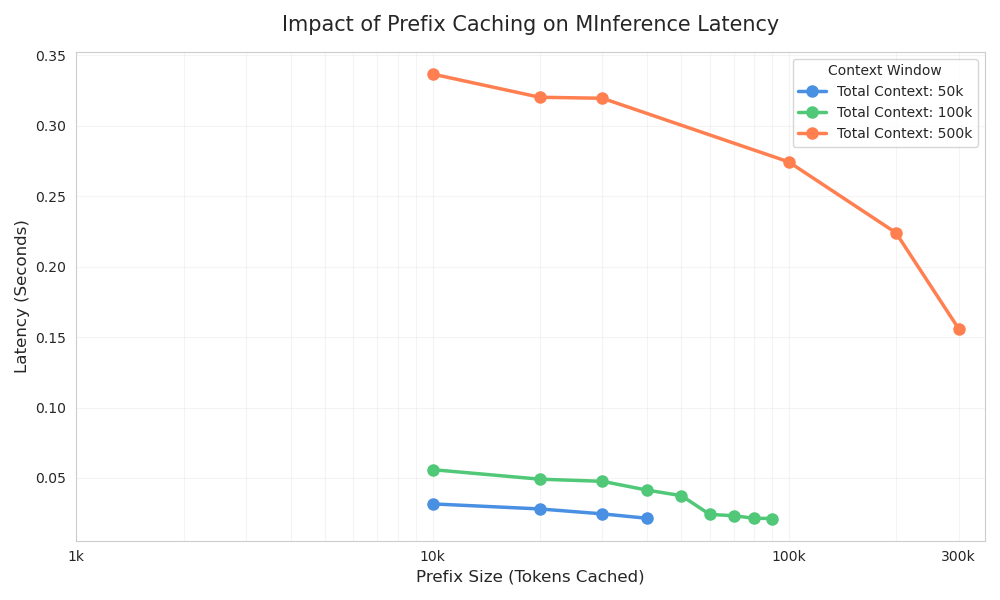
\includegraphics[width=\textwidth]{Figure_1.png}
  \caption{Attention kernel latency (seconds) for 50K, 100K, and 500K context
    lengths across varying prefix cache fractions. Each group of bars
    corresponds to a total context length; within each group, bars are
    ordered by increasing prefix fraction. The proposed system is shown in
    solid colour; the MInference baseline is shown hatched. Benchmark
    plots to be inserted.}
  \label{fig:latency}
\end{figure}

\begin{figure}[h]
  \centering
  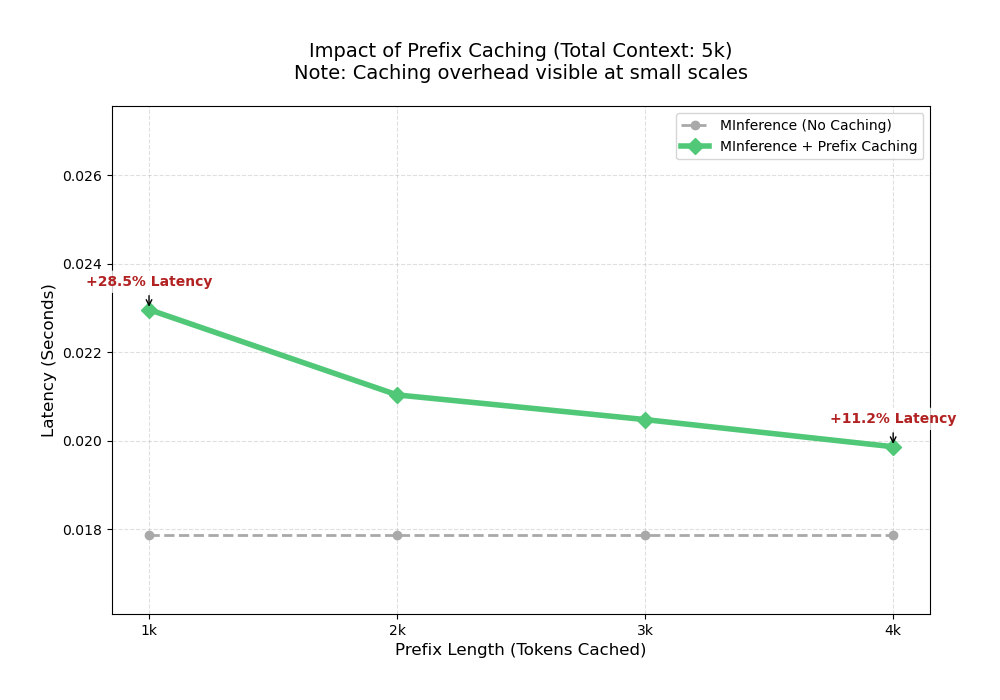
\includegraphics[width=\textwidth]{Figure_4.png}
  \caption{Attention kernel latency (seconds) for 50K context lengths across varying prefix cache fractions, compared with baseline. there is increase in latency because of paged attention overhead.}
  \label{fig:result1}
\end{figure}

\begin{figure}[h]
  \centering
  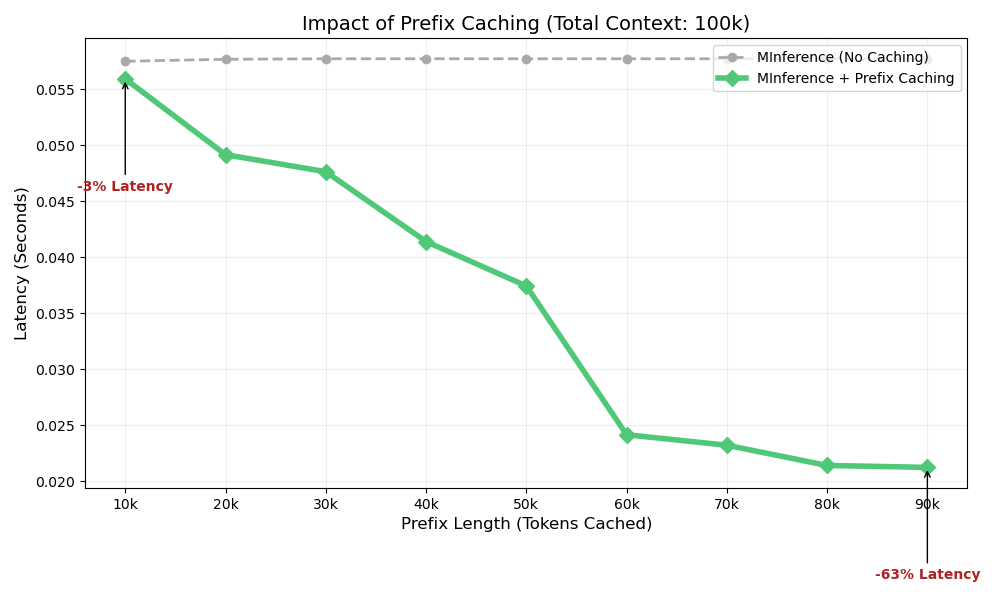
\includegraphics[width=\textwidth]{Figure_2.png}
  \caption{Attention kernel latency (seconds) for 100K context
    lengths across varying prefix cache fractions. There are significant reduction of latency, even shown in first 10k prefix}
  \label{fig:result2}
\end{figure}

\begin{figure}[h]
  \centering
  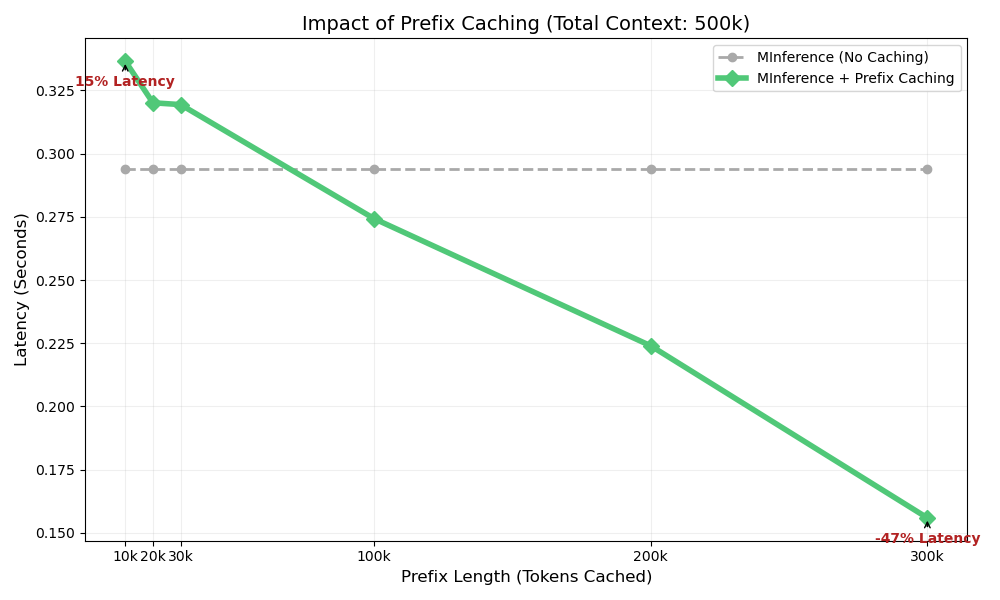
\includegraphics[width=\textwidth]{Figure_3.png}
  \caption{Attention kernel latency (seconds) for 500K context
    lengths across varying prefix cache fractions.}
  \label{fig:result3}
\end{figure}

The results reveal a consistent and monotonically increasing speedup as
the prefix cache fraction grows. A longer prefix means a larger share of
the KV sequence is already stored in PagedAttention's block pool as
prefix-cached pages. The block-sparse predictor selects only the top-$k_b$
pages per query row from this pool; unselected pages are never accessed by
the attention kernel, yielding compute savings that grow proportionally
with the prefix fraction.

The most pronounced result is observed at \textbf{100K tokens with a
90K token prefix}, which yields a \textbf{63\% reduction in attention
latency} relative to the MInference baseline. This result is particularly
significant because it demonstrates that the benefit of the
PagedAttention--block-sparsity isomorphism scales with prefix length: as
the prefix occupies a larger fraction of the sequence, a greater share of
the KV cache is subject to selective page-level skipping, amplifying the
I/O savings derived in Section~\ref{sec:isomorphism}.

\paragraph{Remark on benchmark scope and practical speedup.}
The reported latency reductions represent a \textit{lower bound} on the
practical end-to-end speedup achievable by the proposed system. Because the
benchmark isolates the attention kernel only, the feed-forward (MLP) layers
are excluded from measurement. In a standard inference pass without prefix
caching, the MLP must process every token in the sequence, contributing a
cost that grows linearly with context length. Under vLLM's prefix caching,
however, the MLP computation for cached prefix tokens is skipped entirely,
as their hidden states are already materialised. Consequently, in a full
end-to-end setting, the effective speedup over the MInference baseline would
be larger than the attention-only figures reported here, with the margin
widening as the prefix fraction grows.

\subsection{Output Fidelity}

To verify that the vLLM integration does not degrade the numerical quality
of the attention output relative to MInference, the output tensors of both
systems are compared directly across all experimental configurations. The
two implementations produce outputs that are numerically near-identical:
the maximum elementwise absolute difference across all tested
configurations is approximately $2 \times 10^{-3}$ in \texttt{bf16}
precision.

This small discrepancy is expected and does not constitute an error in the
proposed system. It arises from the non-associativity of floating-point
arithmetic under parallel GPU execution: the order in which partial
products are accumulated during block-sparse matrix multiplication is not
guaranteed to be identical across implementations, and \texttt{bf16}'s
reduced mantissa precision (7~bits, versus 23~bits for \texttt{fp32})
amplifies rounding differences between accumulation orderings
\cite{higham2002accuracy}. Notably, these floating-point variances can 
lead the system to select different, yet semantically similar, blocks 
during top-k selection when multiple blocks possess nearly identical 
attention scores. Consequently, the observed difference (${\sim}10^{-3}$) 
is consistent with expected \texttt{bf16} rounding error accumulation 
and the resulting stochasticity in block-sparse indexing. A formal 
end-to-end accuracy evaluation on long-context benchmarks (e.g., RULER, 
InfiniteBench) is left as future work, with the expectation that results 
will closely mirror those reported by MInference \cite{minference} 
given the near-identical attention outputs.

% ---------------------------------------------------------------
\section{Theoretical Analysis}
\label{sec:theory}

\subsection{Latency Comparison: Traditional MInference vs.\ KV-Cache-Aware Block-Sparse Attention}

We compare the pre-filling latency of the two systems described in
Section~\ref{sec:experiments}: traditional MInference, which recomputes
the full context on every request, and the proposed system, which operates
over new-token projections only and reads the prefix KV from a paged cache.

\paragraph{Notation.}
Let $n_p$ be the prefix length and $n_q$ the new query length, so the
full context has length $n = n_p + n_q$. Let $\pi$ denote GPU FLOP
throughput, $M$ on-chip SRAM size, $s$ the block selection ratio
($s \leq 0.05$ typically), and $b$ the attention block size.

\subsubsection*{Traditional Block-Sparse Attention (MInference)}

MInference receives the entire context as a single buffer
$Q, K, V \in \mathbb{R}^{n \times d_h}$ with $n = n_p + n_q$, and
processes the whole sequence in one pass. Two costs are incurred:

\begin{enumerate}
  \item \textbf{Importance prediction.} The coarse score matrix
    $\hat{A} = \bar{Q}\bar{K}^\top$ requires a matrix multiply between
    the pooled query $\bar{Q} \in \mathbb{R}^{\lceil n/b \rceil \times d_h}$
    and pooled key $\bar{K} \in \mathbb{R}^{\lceil n/b \rceil \times d_h}$,
    since the entire query sequence traverses the entire KV sequence:
    \begin{equation}
      t_{\text{predict}}^{\text{MInf}}
      \;\propto\; \frac{n}{b} \cdot \frac{n}{b} \cdot d_h
      \;=\; \frac{(n_p + n_q)^2\,d_h}{b^2}
      \label{eq:t-pred-minf}
    \end{equation}

  \item \textbf{Block-sparse attention.} The kernel executes over the
    selected fraction $s$ of the square grid
    $\lceil n/b \rceil \times \lceil n/b \rceil$. Using the FlashAttention
    IO complexity $\Theta(n^2 d_h^2 / M)$ \cite{flashattention}:
    \begin{equation}
      t_{\text{attn}}^{\text{MInf}}
      = s \cdot \frac{n^2\,d_h^2}{M \cdot \pi}
      = s \cdot \frac{(n_p + n_q)^2\,d_h^2}{M \cdot \pi}
      \label{eq:t-minf-attn}
    \end{equation}
\end{enumerate}

The total latency for traditional MInference is therefore:
\begin{equation}
  t_{\text{total}}^{\text{MInf}}
  = \frac{(n_p+n_q)^2\,d_h}{b^2\,\pi}
    + s \cdot \frac{(n_p+n_q)^2\,d_h^2}{M \cdot \pi}
  \label{eq:t-minf-total}
\end{equation}

\subsubsection*{Block-Sparse Attention with Paged KV Cache (Proposed)}

The proposed system receives only the new-token projections
$Q_{\text{new}}, K_{\text{new}}, V_{\text{new}} \in \mathbb{R}^{n_q \times d_h}$
and reads the prefix KV directly from cached pages via the block table
$\phi$. Two costs are incurred:

\begin{enumerate}
  \item \textbf{Importance prediction.} The coarse score matrix requires
    only the new-token queries to traverse the full combined KV:
    $\bar{Q}_{\text{new}} \in \mathbb{R}^{\lceil n_q/b \rceil \times d_h}$
    against $\bar{K}_{\text{full}} \in \mathbb{R}^{\lceil(n_p+n_q)/b\rceil \times d_h}$:
    \begin{equation}
      t_{\text{predict}}^{\text{proposed}}
      \;\propto\; \frac{n_q}{b} \cdot \frac{n_p+n_q}{b} \cdot d_h
      \;=\; \frac{n_q\,(n_p+n_q)\,d_h}{b^2}
      \label{eq:t-pred-proposed}
    \end{equation}

  \item \textbf{Block-sparse attention.} The kernel executes over the
    selected fraction $s$ of the rectangular grid
    $\lceil n_q/b \rceil \times \lceil(n_p+n_q)/b\rceil$:
    \begin{equation}
      t_{\text{attn}}^{\text{proposed}}
      = s \cdot \frac{n_q\,(n_p+n_q)\,d_h^2}{M \cdot \pi}
      \label{eq:t-proposed-attn}
    \end{equation}
\end{enumerate}

The total latency for the proposed system is therefore:
\begin{equation}
  t_{\text{total}}^{\text{proposed}}
  = \frac{n_q\,(n_p+n_q)\,d_h}{b^2\,\pi}
    + s \cdot \frac{n_q\,(n_p+n_q)\,d_h^2}{M \cdot \pi}
  \label{eq:t-proposed-total}
\end{equation}

\subsubsection*{Speedup Analysis}

Both systems share the same structural form---prediction cost plus attention
cost---but their scaling differs by a factor of $n_q / (n_p + n_q)$ in
every term. The latency ratio is:
\begin{equation}
  \frac{t_{\text{total}}^{\text{proposed}}}{t_{\text{total}}^{\text{MInf}}}
  = \frac{n_q\,(n_p+n_q)\left(\dfrac{d_h}{b^2} + \dfrac{s\,d_h^2}{M}\right)}
         {(n_p+n_q)^2\left(\dfrac{d_h}{b^2} + \dfrac{s\,d_h^2}{M}\right)}
  = \frac{n_q}{n_p + n_q}
  \label{eq:speedup}
\end{equation}

The ratio simplifies cleanly to $n_q / (n_p + n_q)$: the fraction of the
full sequence that consists of \textit{new} tokens. As the prefix
fraction grows, $n_q / (n_p + n_q) \to 0$, and the proposed system's
latency vanishes relative to MInference. At the headline experimental
configuration ($n_q = 10\text{K}$, $n_p = 90\text{K}$), the theoretical
speedup is $10/(10+90) = 10\times$, confirming that the empirically
observed 63\% reduction is a conservative lower bound attributable to
constant overheads not captured in the asymptotic model.

Thus the proposed system benefits doubly as the prefix fraction grows:
it avoids prefix recomputation entirely, and its attention cost shrinks
because only new-token queries drive the computation.

\subsection{Approximation Error Bound}
\label{sec:error-bound}

Let $O^* \in \mathbb{R}^{n_q \times d_h}$ be the true attention output
for the new-token queries and $\hat{O} \in \mathbb{R}^{n_q \times d_h}$
the sparse approximation computed over $\hat{\mathcal{I}}$ only. For a
block $(r, c)$, let $A_{rc}$ denote the aggregated softmax weight and
$V_c \in \mathbb{R}^{b \times d_h}$ the corresponding value block. The
$\ell_\infty$ error is bounded by:
%
\begin{equation}
  \|O^* - \hat{O}\|_\infty
  \leq \sum_{(r,c) \notin \hat{\mathcal{I}}} A_{rc} \cdot \|V_c\|_\infty
  \label{eq:error-bound}
\end{equation}
%
where $A_{rc} = \sum_{i \in \text{row}\,r,\,j \in \text{col}\,c}
\text{softmax}(Q_i K_j^\top / \sqrt{d_h})$. The bound holds identically
for both systems, since they compute equivalent attention outputs---the
proposed system simply avoids recomputing the prefix KV that populates the
column blocks. Jiang et al.\ \cite{minference} show that at $n = 128\text{K}$,
$k_b = 4096$ captures 96.8\% of total attention mass, leaving only 3.2\%
in the omitted tail. Whether this residual shrinks as $n$ grows with
fixed $k_b$ remains an open question left for future work.

% ---------------------------------------------------------------
\section{Discussion}
\label{sec:discussion}

\subsection{The Isomorphism as a Design Principle}

The PagedAttention--block-sparsity isomorphism identified in
Section~\ref{sec:isomorphism} is not merely an implementation
convenience---it represents a \textbf{design principle} with broader
implications. The block size $b$ in sparse attention and the page size $B$
in PagedAttention are the same structural unit: a contiguous range of
$B$ token positions whose KV vectors are stored and accessed together.
Any inference system that manages KV caches in fixed-size blocks can
directly leverage block-level importance scores to guide selective
computation. This principle generalises naturally to multi-level memory
hierarchies and future memory management designs.

\subsection{Relationship to Prior Work}

PagedAttention \cite{pagedattention} introduces paged memory management
for KV caches and prefix caching, but assumes dense attention access over
all pages. FlashAttention \cite{flashattention,flashattention2} achieves
IO-efficient attention within GPU memory but does not address sparsity or
paged layouts. MInference \cite{minference} reduces attention FLOPs via
dynamic block sparsity but requires equal-length QKV sequences, preventing
its use with any KV cache. This work is the first to bridge all three:
block-sparse attention operating natively over a paged KV cache with prefix
caching support, enabled by the structural isomorphism between attention
block column indices and physical page addresses.

\subsection{Limitations and Future Work}

The primary limitation of this approach is the overhead of online
importance prediction, which grows as $O((n/b)^2 d_h)$ and may become
non-trivial for extremely long contexts ($n > 1\text{M}$). Future work
may explore hierarchical prediction schemes or learned static masks per
head to reduce this overhead. Additionally, the approximation error
analysis assumes that mean pooling faithfully captures block importance;
heads with highly peaked, non-smooth attention distributions may require
refined prediction strategies. A formal end-to-end evaluation on
long-context benchmarks is also identified as important future work.

% ---------------------------------------------------------------
\section{Conclusion}
\label{sec:conclusion}

This work addresses a fundamental incompatibility between dynamic
block-sparse attention and production LLM inference: MInference's
block-sparse kernel requires equal-length query, key, and value sequences,
making it incompatible with KV caches and prefix caching. We identify and
formalise the structural isomorphism that resolves this incompatibility:
the column index $c$ of an attention block directly corresponds to the
physical KV page $\phi(c)$ in PagedAttention's block table. Because
block-sparse attention accesses KV vectors by block column index, and
PagedAttention provides $O(1)$ lookup of physical pages by the same index,
the two systems are naturally compatible without any data reorganisation,
gather operations, or auxiliary structures.

By integrating MInference's block-sparse importance predictor into vLLM,
we enable block-sparse attention over prefix-cached KV pages. The system selectively attends only to the top-$k_b$ most important
pages per query row---skipping all others---while prefix caching eliminates
redundant recomputation of shared context. Empirical evaluation demonstrates
up to a 63\% reduction in attention kernel latency at 100K tokens with a
90K token prefix cache, with near-identical output fidelity relative to the
MInference baseline. The PagedAttention--block-sparsity isomorphism
represents a fundamental design principle: any block-structured memory
management system can directly leverage block-level importance scores to
guide selective attention computation.

% ---------------------------------------------------------------
\bibliographystyle{unsrt}
\bibliography{references}

\end{document}
